\documentclass[a4paper,12pt]{article}

\usepackage[slovene]{babel}
\usepackage{amsfonts,amssymb,amsmath, mathtools}
\usepackage[utf8]{inputenc}
\usepackage[T1]{fontenc}
\usepackage{lmodern}
\usepackage{graphicx}


\def\R{\mathbb{R}} % mnozica realnih stevil

\def\qed{$\hfill\Box$}   % konec dokaza
\def\qedm{\qquad\Box}   % konec dokaza v matematičnem načinu



\title{Krožnica v racionalni Bezierjevi obliki \\ 
\Large Seminar pri predmetu RPGO}
\author{Samo Kralj, Anja Kišek \\
Fakulteta za matematiko in fiziko}
\date{januar 2019}

\begin{document}
%%%%%%%%%%%%%%%%%%%%%%%%%%%%%%%%%%%%
\maketitle
\section{Uvod}
V seminarski nalogi bova predstavila racionalne Bezierjeve krivulje ter njihovo uporabo pri risanju krožnic in krožnih lokov. Za razliko od polinomskih Bezierjevih krivulj, ki krožni lok lahko le poljubno dobro aproksimirajo, ga racionalne krivulje opišejo eksaktno. Pri njihovi obravnavi se je zavoljo implementacije in uporabe koristno osredotočiti na pozitivnost uteži krivulje, zato se bova poskušala omejiti le na primere, kjer se to da doseči.

V prvem poglavju bova predstavila racionalne Bezierjeve krivulje ter nekaj njihovih lastnosti. Drugo poglavje bo namenjeno konstrukciji sklenjene krožnice s pomočjo racionalne krivulje čim nižje stopnje, v tretjem pa bova ugotovljeno aplicirala na primeru krožnih lokov s pozitivnimi utežmi. Zadnje poglavje bo opisovalo uporabo izpeljanega na kubičnih polkrogih ter podalo geometrijsko konstrukcijo pripadajočega kontrolnega poligona.

\section{Racionalne Bezierjeve krivulje}
Racionalna Bezierjeva krivulja $C(t)$ stopnje $n$ v $\mathbb{R}^d$ je projekcija polinomske Bezierjeve krivulje $\tilde{C}(t)$stopnje $n$ v $\mathbb{R}^{d+1}$ na hiperravnino $w=1$, kjer je točka v $\mathbb{R}^{d+1}$ označena z $
\begin{bmatrix} x \\ w \end{bmatrix}.$ Racionalna B. krivulja stopnje $n$ je tako podana s predpisom
$$r(t) = \frac{\sum_{i=0}^n w_ib_iB_i^n(t)}{\sum_{i=0}^n w_iB_i^n(t)}, $$
kjer je $B_i^n(t)$ i-ti Bernsteinov bazni polinom stopnje $n$, $b_i$ kontrolne točke krivulje, $w_i$ pa uteži.

Racionalna krivulja $C(t) = (X(t), Y(t))$ lahko eksaktno opiše krožnico kot projekcijo krivulje
$\tilde{C}(t) = (\tilde{X}(t), \tilde{Y}(t), W(t)),$ ki leži na stožcu $$\tilde{X}(t)^2 + \tilde{Y}(t)^2 - W(t)^2 = 0,$$ na ravnino $w = 1$. Slednje nam pokaže naslednji račun:

\begin{align*}
X(t)^2 + Y(t)^2 &= 1 \\
\Big{(}\frac{\tilde{X}(t)}{W(t)}\Big{)}^2 + \Big{(}\frac{\tilde{Y}(t)}{W(t)}\Big{)}^2 &= 1\\
\tilde{X}(t)^2 + \tilde{Y}(t)^2 - W(t)^2 &= 0
\end{align*}
Prva enačba predstavlja enačbo krožnice v prostoru $\mathbb{R}^2$, nato pa koordinate točk zamenjamo za tiste iz prostora $\mathbb{R}^3$, dobljene s projekcijo na ravnino $w=1$. Izraz lahko preoblikujemo v zadnjo enačbo, ki podaja običajno enačbo stožca.

\begin{figure}[h!]
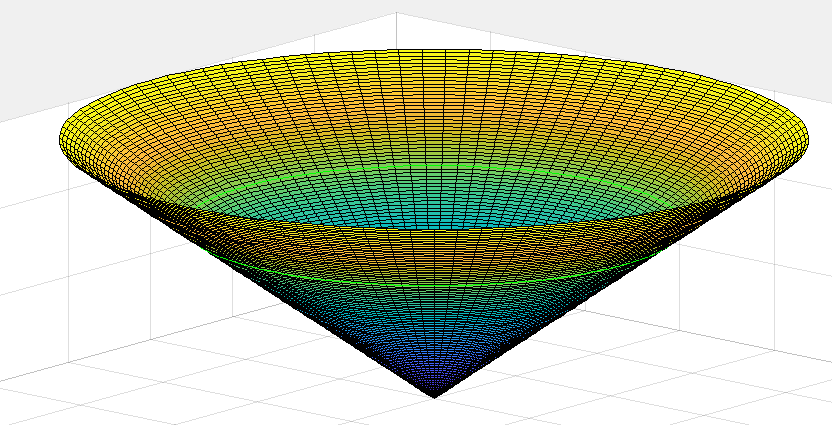
\includegraphics[scale=0.25]{stozec.png}
\centering
\caption{Stožec $\tilde{X}(t)^2 + \tilde{Y}(t)^2 - W(t)^2 = 0$, s katerega se vse krivulje projicirajo na krožnico v ravnini $w=1$.}
\end{figure}

Problem iskanja racionalne krivulje, ki opiše krožnico oziroma krožni lok, lahko prevedemo na iskanje krivulje, ki leži na omenjenem stožcu. Pogoj pozitivnih uteži lahko geometrijsko interpretiramo kot pogoj, da kontrolni poligon leži v zgornji polravnini $w > 0$.

\section{Bezierjeva krivulja kot sklenjena krivulja}
V tem poglavju si bomo ogledali, kako krožnico opišemo z eno samo racionalno krivuljo (in ne zlepkom krivulj) ter kakšna je najmanjša stopnja krivulje, s katero to lahko dosežemo.

\subsection{Kvadratična krivulja}
Ali se sklenjeno krožnico da opisati s krivuljo stopnje dve? Da to ni mogoče, se hitro prepričamo z naslednjim razmislekom: vsaka krivulja stopnje 2 je parabola; vsako parabolo, ki leži na stožcu, pa dobimo s presekom stožca z ravnino, ki je vzporedna nosilki stožca. Opazimo, da bolj, kot bomo ravnino približevali nosilki stožca, večji kot bo opisal krožni lok v projekciji. Vendar ko se ravnina in stožec stakneta, je presečišče zgolj premica, ta pa se v projekciji slika v eno samo točko. Krožnice zato ne moremo predstaviti s kvadratično racionalno krivuljo.

\begin{figure}[h]
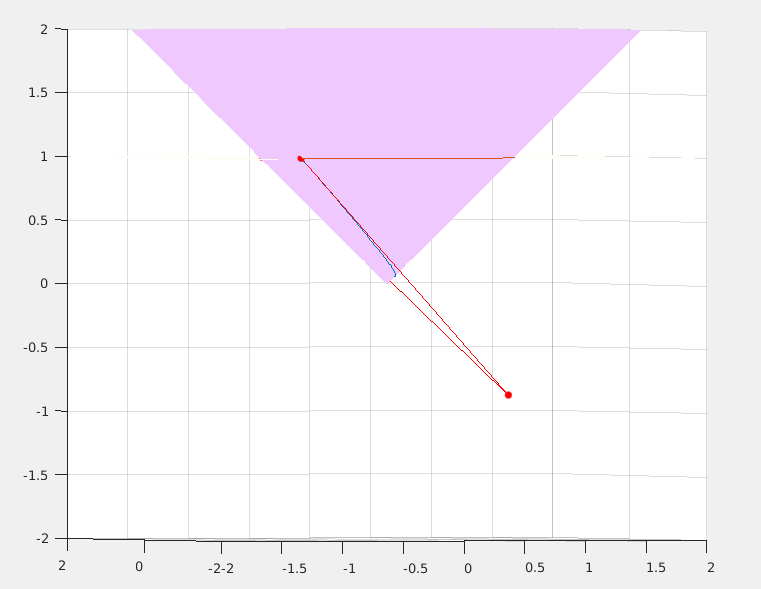
\includegraphics[scale=0.25]{kvadraticna.png}
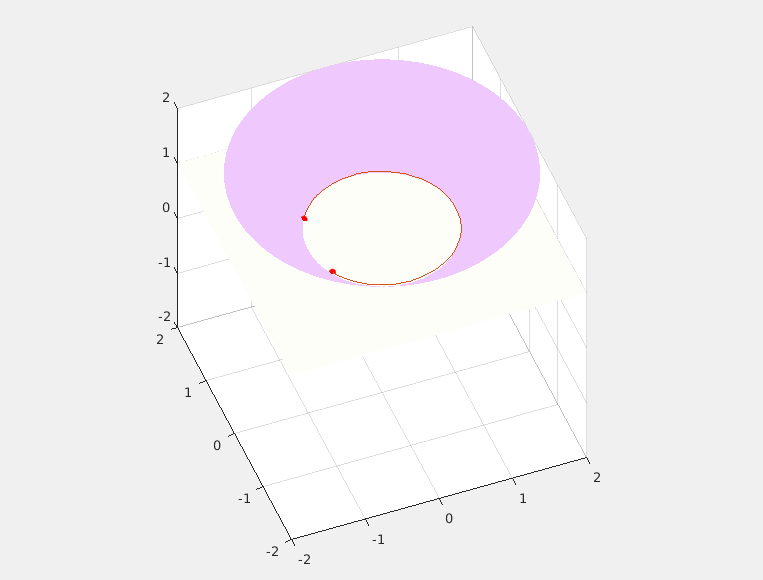
\includegraphics[scale=0.25]{kvadraticna2.png}
\centering
\caption{Parabola, dobljena kot presek ravnine in stožca, ki se preslika v krožni lok.}
\end{figure}

Očitno z dobljeno parabolo lahko opišemo krožne loke, zato si oglejmo, kako zgleda kontrolni poligon takšne krivulje. Za prvo in zadnjo točko si izberemo točki, ki ležita na krožnici, srednjo točko pa zaradi simetrije izberemo na polovičnem kotu med njima. Pri tem izberemo take uteži, da zadoščajo enačbi stožca. Klasičen kontrolni poligon za polovični kot krožnega loka $\phi$ je tedaj:
\begin{align*}
\tilde{P}_0 &= (cos(\phi), -sin(\phi), 1)\\
\tilde{P}_1 &= (1, 0, cos(\phi))\\
\tilde{P}_2 &= (cos(\phi), sin(\phi), 1).
\end{align*}

\subsection{Kubična krivulja}
Izkaže se, da tudi kubična krivulja ne more opisati sklenjene krožnice. Oglejmo si, zakaj.

Za kontrolni poligon moramo izbrati štiri točke. Krivulja interpolira prvo in zadnjo točko, zato ju izberemo na stožcu. Ker je krivulja sklenjena in ker ju bo projekcija preslikala v isto točko na ravnini $w=1$, si brez škode za splošnost izberemo kar to točko na ravnini. Da bo krivulja ležala na tangenti, morata druga in tretja točka ležati na tangentni ravnini stožca v prvi/zadnji točki. Tako dobimo štiri točke, ki vse ležijo na isti ravnini, po lastnosti Bezierjevih krivulj, ki ležijo v konveksni ovojnici kontrolnega poligona, pa zaključimo, da je dobljena krivulja lahko le točka.

\subsection{Krivulja stopnje 4}
Pri krivulji četrte stopnje je svobode pri izbiranju točk na kontrolnem poligonu več, zato si izberimo drugačen pristop. V enačbo $$\tilde{X}(t)^2 + \tilde{Y}(t)^2 - W(t)^2 = 0$$ po komponentah vstavimo enačbo $$B^4(t) = \sum_{i=0}^4b_iB_i^4(t).$$

mogoče bi semle premaknil tisto ugotovitev, kako se Bernsteinovi množijo med sabo?

Ker so Bernsteinovi polinomi baza prostora, bo enakost veljala, ko bo seštevek koeficientov pred $i$-tim polinomom enak 0. Upoštevamo še, da lahko prvo in zadnjo točko postavimo na $\tilde{P}_0 = (1,0, 1), \tilde{P}_4 = (1,0, 1)$ ter da druga in predzadnja točka ležita v tangentni ravnini $\tilde{P}_0$, to je ravnini $x = w$. S tem se prejšnjih devet enačb poenostavi v naslednjih pet:
\begin{align*}
\tilde{y}_3 + \tilde{y}_1 &= 0\\
\tilde{x}_3 + \tilde{x}_1 &= 0\\
3\tilde{x}_2 + 4\tilde{y}_1^2 - 3w_3 &= 0 \\
\tilde{x}_1\tilde{x}_2 + \tilde{y}_1\tilde{y}_2  - \tilde{x}_1w_2 &= 0 \\
9\tilde{x}_2^2 - 8\tilde{y}_1^2 + \tilde{y}_2^2 - 9w_2^2&= 0 \\
\end{align*}
Zaradi potenc stopnje dve ne dobimo enolične rešitve, temveč dva možna kontrolna poligona. Za $\alpha = (\frac{3w_2}{2} - \tilde{x}_1^2 + \frac{1}{2})^{\frac{1}{2}}$ dobimo dve poenostavljeni rešitvi:
\begin{align*}
\tilde{P}_0 &= (1,0, 1)\\
\tilde{P}_1 &= (\tilde{x}_1, \pm \alpha,\tilde{x}_1)\\
\tilde{P}_2 &= (-\frac{3w_2 - 4\tilde{w}_1^2+2}{3}, \pm \frac{3}{4}\tilde{x}_1\alpha, w_2)\\
\tilde{P}_3 &= (-\tilde{x}_1, \mp \alpha,-\tilde{x}_1)\\
\tilde{P}_4 &= (1,0,1) \\
\end{align*}
Da bo $\alpha$ realno število, morata veljati neenakosti $$w_2 > -\frac{1}{3}$$ in $$-\Big{(}\frac{3w_2+1}{2}\Big{)}^{1/2} < \tilde{x}_1 < \Big{(}\frac{3w_2+1}{2}\Big{)}^{1/2}.$$
Opazimo, da ne glede na izbor $w_2$ in $\tilde{x}_1$ uteži nikoli ne bodo vse pozitivne.
\begin{figure}[h!]
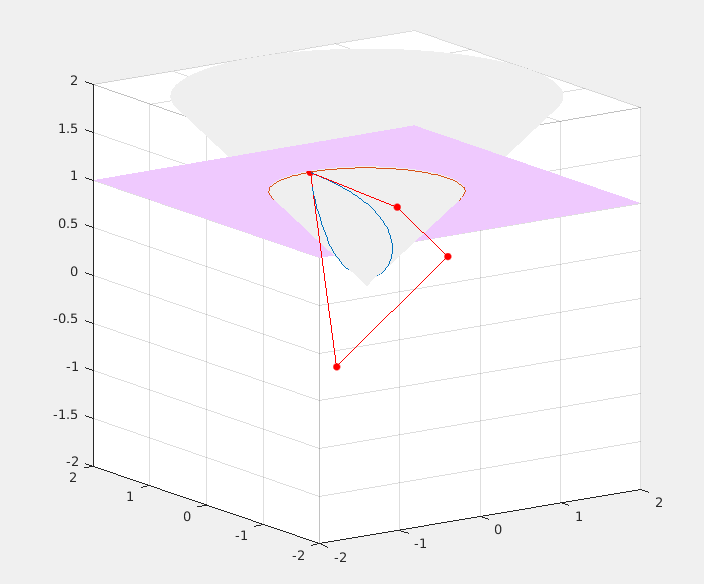
\includegraphics[scale=0.35]{kvarticna.png}
\centering
\caption{Krožnica pri krivulji stopnje 4 pri izbranem $w_2 = 1/3$ in $\tilde{x}_1 = -\Big{(}\frac{3w_2+1}{2}\Big{)}^{1/2} + 0.8 \Big{(}\frac{3w_2+1}{2}\Big{)}^{1/2}$.}
\end{figure}

Oglejmo si, kaj se zgodi, če izberemo $\tilde{x}_1=0$. Tedaj nimamo več negativnih uteži, imamo pa dve ničelni. Točki v kontrolnem poligonu, za kateri velja $w=0$, pri projekciji na ravnino $w=1$ predstavljata točki v neskončnosti, česar si pri implementaciji in uporabi ne želimo.
\begin{figure}[h]
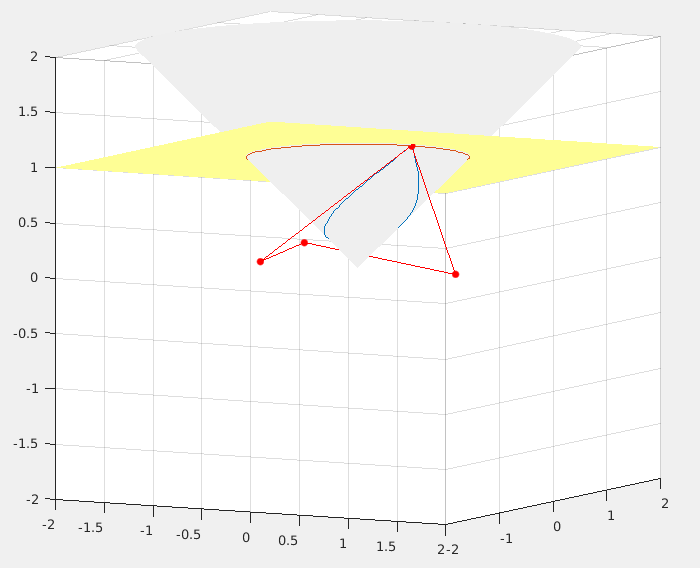
\includegraphics[scale=0.24]{nicelneutezi.png}
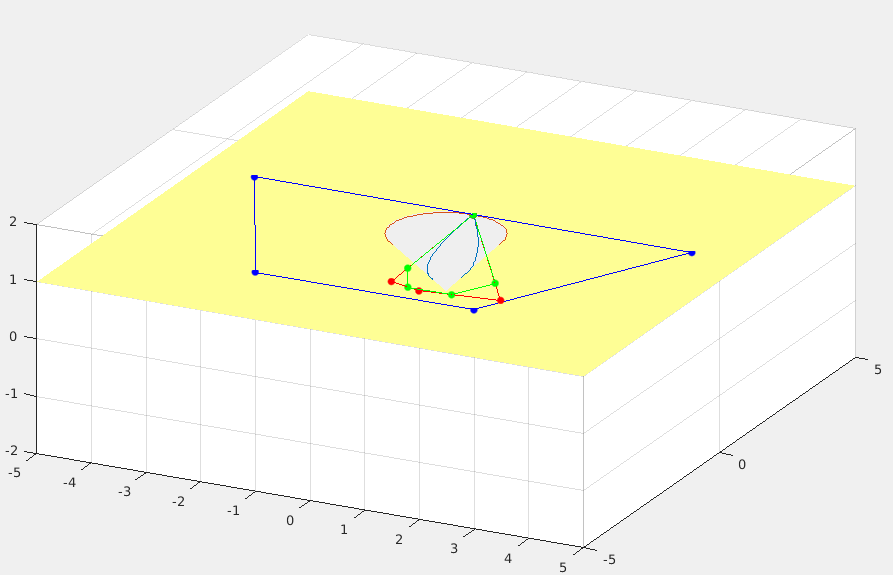
\includegraphics[scale=0.24]{kvinticna.png}
\centering
\caption{Levo: krožnica pri krivulji stopnje 4 z dvema ničelnima utežema in desno: ista krivulja z dvignjeno stopnjo, ki ima vse uteži pozitivne.}
\end{figure}
Težave odpravimo, če dani krivulji dvignemo stopnjo -- krivulja ostane enaka, kontrolni poligon pa se pomakne bliže krivulji. Izkaže se, da so pogoji za obstoj take krivulje tedaj $$-\frac{1}{4} < \tilde{x}_1 < \frac{1}{4}$$ in $$-\frac{2}{3}w_2 < \tilde{x}_1 <  \frac{2}{3}w_2.$$
Za primer na sliki 4 je izbran kontrolni poligon z dvema ničelnima utežema, nato pa je z dvigom stopnje dobljen desni poligon, ki nima več nepozitivnih uteži.

\begin{equation*}
\begin{aligned}[c]
\tilde{P}_0 &= (1,0, 1)\\
\tilde{P}_1 &= (0, 1, 0)\\
\tilde{P}_2 &= (-1, 0, 1/3)\\
\tilde{P}_3 &= (0, -1, 0)\\
\tilde{P}_4 &= (1, 0, 1), \\
\end{aligned}
\begin{aligned}[c]
\tilde{P}_0 &= (1,0, 1)\\
\tilde{P}_1 &= (1/5, 4/5, 1/5)\\
\tilde{P}_2 &= (-3/5, 2/5, 1/5)\\
\tilde{P}_3 &= (-3/5, -2/5, 1/5)\\
\tilde{P}_4 &= (1/5, -4/5, 1/5)\\
\tilde{P}_5 &= (1, 0, 1). \\
\end{aligned}
\end{equation*}




\end{document}